%%%%%%%%%%%%%%%%%%%%%%%%%%%%%%%%%%%%%%%%%%%%%%%%%%%%%%% 
% Please note that whilst this template provides a 
% preview of the typeset manuscript for submission, it 
% will not necessarily be the final publication layout.
%
% letterpaper/a4paper: US/UK paper size toggle
% num-refs/alpha-refs: numeric/author-year citation and bibliography toggle

\documentclass[a4paper,num-refs,gigabyte,usenames,dvipsnames]{oup-contemporary}

%%% Journal toggle; only specific options recognised.
%%% (Only "gigabyte", "gigascience" and "general" are implemented now. Support for other journals is planned.)
\journal{gigabyte}


\usepackage{siunitx}
\usepackage{pbox, calc}
\usepackage{marginnote}



\usemintedstyle{igor}

%%% Flushend: You can add this package to automatically balance the final page, but if things go awry (e.g. section contents appearing out-of-order or entire blocks or paragraphs are coloured), remove it!
% \usepackage{flushend}

\def\flushRight{\leftskip0pt plus 1fill\rightskip0pt}

\title{Audit Report for: Customer}

%%% Use the \authfn to add symbols for additional footnotes, if any. 1 is reserved for correspondence emails; then continuing with 2 etc for contributions.
\author[1,\authfn{1},\authfn{2}]{to: customer}



%%% Author Notes
\authnote{\authfn{1}from: mishellcode@unicornsecurity.io}

%%% "Short" author for running page header
\runningauthor{Antoine Royer, Nathalie Cochard}

%%% Should only be set by an editor
\jvolume{00}
\jnumber{0}
\jyear{2020}

\iffalse

\begin{theo}[{\vulntype}]{}
  \begin{center}
    \begin{tabular}{l p{0.7\linewidth}}    
      \textbf{\texttt{\vulntype\thevuln}} & \textbf{} \\\midrule
      Description    & 
      \\ 
      \midrule
      Impact & 
      \\ \midrule
      \rowcolor{Orange!50} Criticity & Medium
      \\ \midrule
      \rowcolor{green!20} Mitigation & 
      \\
      \bottomrule
      \hline
    \end{tabular}
  \end{center}
\end{theo}

\fi

\definecolor{lightpurple}{HTML}{F2E4FF}
\definecolor{subtlegray}{HTML}{EAEAEA}

 \lstdefinestyle{tree}{
    literate=
    {├}{{\smash{\raisebox{-1ex}{\rule{1pt}{\baselineskip}}}\raisebox{0.5ex}{\rule{1ex}{1pt}}}}1 
    {─}{{\raisebox{0.5ex}{\rule{1.5ex}{1pt}}}}1 
    {└}{{\smash{\raisebox{0.5ex}{\rule{1pt}{\dimexpr\baselineskip-1.5ex}}}\raisebox{0.5ex}{\rule{1ex}{1pt}}}}1 
  }

\begin{document}

\begin{frontmatter}
\maketitle
\begin{abstract}
Welcome to your Unicorn Security Audit Report. You will find in this document the results of the analysis submitted to Unicorn Security. 
\begin{center}
  \begin{tabular}{|l|c|}
    \hline
    Author&Antoine Royer\\ \hline
    Reviewer&Nathalie Cochard\\ \hline
    Receiving Party&Customer \\ \hline
  \end{tabular}
\end{center}

\end{abstract}
\end{frontmatter}

\section{Summary}
\setcounter{note}{0}
%\input{summary.tex}
\section{System Level Vulnerabilities}

\setcounter{vuln}{0}
\def \vulntype {SYS}

\marginnote{
  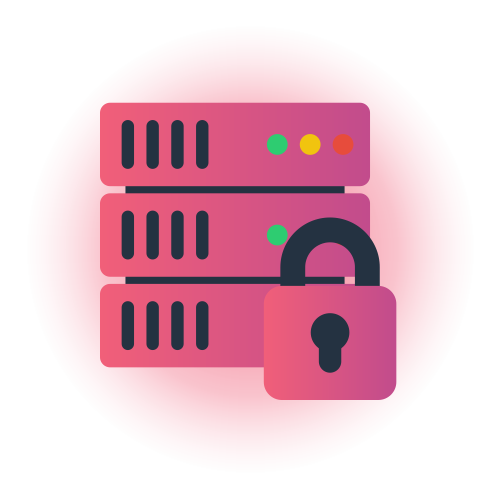
\includegraphics[width=30px]{icons/system.png}
}[-31px]

%\input{sys.tex}
\section{\raggedright Application Level Vulnerabilities}

\setcounter{vuln}{0}
\def \vulntype {APP}

\marginnote{
  
\includegraphics[width=30px]{icons/web.png}
}[-31px]

%\input{app.tex}
\section{Cryptography}

\setcounter{vuln}{1}
\def \vulntype {CRYPT}

\marginnote{
  
\includegraphics[width=30px]{icons/crypto.png}
}[-31px]
%\input{crypto.tex}
\tableofcontents

\end{document}
